%Segunda Unidad
\section{Aproximación de funciones}
\begin{frame}[allowframebreaks]{Mínimos cuadrados}
Considere el siguiente conjunto de datos $\{(x_i,y_i)\}_{i=1}^{N}$ asociados:
\begin{displaymath}
\begin{bmatrix}
1&2&3&4&5&6&7&8&9&10\\
\downarrow &\downarrow &\downarrow &\downarrow &\downarrow &\downarrow &\downarrow &\downarrow &\downarrow &\downarrow\\
3&5&9&11&15&17&20&24&26&29
\end{bmatrix}
\end{displaymath}
Abajo se aprecian los pares ordenados correspondientes a cada par asociado:
\begin{figure}[H]
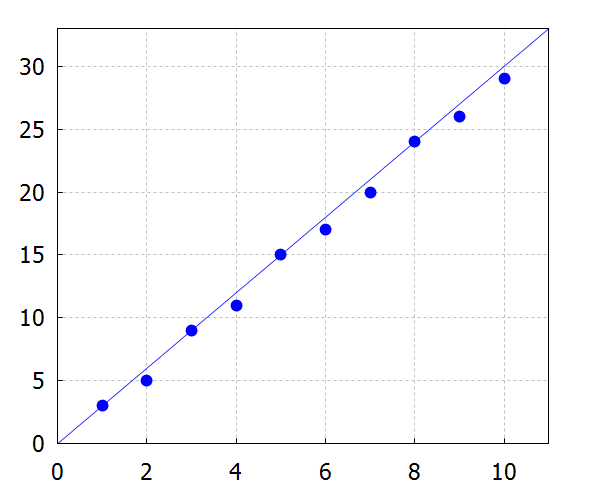
\includegraphics[scale=0.55]{Imagen2}
\caption{Recta de aproximación a los pares ordenados.}
\end{figure}
\indent El objetivo consiste en determinar la recta $Y=a_1X+a_0$ que mejor modele al conjunto de datos asociados.\\
\indent Existen algunos enfoques para encontrar esta recta:
\begin{block}{Problema Minimax}
\centering $\displaystyle \min_{a_0,a_1}\max_{1\leq i\leq 10}|y_i-(a_1x_i-a_0)|$
\end{block}
\begin{block}{Problema de desviación absoluta}
\centering $\displaystyle \min_{a_0,a_1}\sum_{i=1}^{10}|y_i-(a_1x_i-a_0)|$
\end{block}
\begin{block}{Problema de mínimos cuadrados}
\centering $\displaystyle \min_{a_0,a_1}\sum_{i=1}^{10}|y_i-(a_1x_i-a_0)|^2=\displaystyle \min_{a_0,a_1}\sum_{i=1}^{10}(y_i-(a_1x_i-a_0))^2$
\end{block}
\end{frame}
\begin{frame}{Deducción del método de mínimos cuadrados}
Defina los siguientes vectores:
$$X=[x_1,\cdots,x_n]^T$$
$$Y=[y_1,\cdots,y_n]^T$$
$$U=[1,\cdots,1]^T$$
Entonces podemos pensar en el problema de ajuste de la siguiente manera: Deseamos encontrar $a_0$ y $a_1$ tales que
$$a_1X+a_0U=Y$$
De forma matricial esto sería:
\begin{displaymath}
(X|U)
\left(
\begin{array}{c}
a_1\\
a_0
\end{array}
\right)=Y
\end{displaymath}
\end{frame}
\begin{frame}{Deducción del método de mínimos cuadrados}
Si ahora se multiplica por la transpuesta de la primer matriz, se obtine:
\begin{displaymath}
\left(
\begin{array}{c}
X^T\\
U^T
\end{array}
\right)
(X|U)
\left(
\begin{array}{c}
a_1\\
a_0
\end{array}
\right)=
\left(
\begin{array}{c}
X^T\\
U^T
\end{array}
\right)
Y
\end{displaymath}
Esto es equivalente a lo siguiente:
\begin{displaymath}
\left(
\begin{array}{cc}
X^TX &X^TU\\
U^TX & U^TU
\end{array}
\right)
\left(
\begin{array}{c}
a_1\\
a_0
\end{array}
\right)=
\left(
\begin{array}{c}
X^TY\\
U^TY
\end{array}
\right)
\end{displaymath}
Como se puede apreciar, resolviendo este sistema podemos encontrar las soluciones para los coeficientes de la regresión lineal.
\end{frame}
\begin{frame}{Generalización a ajustes de tipo polinomial.}
Ahora considere le problema siguiente: Se desan encontrar los valores $[a_m,a_{m-1},\cdots,a_0]$ de manera tal que:
$$a_mX^m+\cdots+a_1X+a_0U=Y$$
Donde $X^k=[x_1^k,\cdots,x_n^k]^T$. Nuevamente esto se puede escribir como el siguiente sistema:
\textcolor{red}{
\begin{displaymath}
(X^m|X^{m-1}|\cdots X|U)
\left(
\begin{array}{c}
a_m\\
\vdots\\
a_0
\end{array}
\right)=Y
\end{displaymath}
}
Multiplicando por la transpuesta...
\end{frame}
\begin{frame}{Generalización de ajuste  de tipo polinomial}
\begin{displaymath}
\left(
\begin{array}{c}
(X^m)^T\\
\vdots\\
(X)^T\\
U^T
\end{array}
\right)
(X^m|X^{m-1}|\cdots X|U)
\left(
\begin{array}{c}
a_m\\
\vdots\\
a_0
\end{array}
\right)=
\left(
\begin{array}{c}
(X^m)^T\\
\vdots\\
(X)^T\\
U^T
\end{array}
\right)
Y
\end{displaymath}
Lo que termina siendo equivalente a resolver el sistema:
\begin{displaymath}
\left(
\begin{array}{cccc}
(X^m)^TX^m & (X^m)^TX^{m-1} &\hdots & (X^m)^TU\\
\vdots&\vdots &&\vdots\\
(X)^TX^m&(X)^TX^{m-1}&\hdots &(X)^TU\\
U^TX^m&U^TX^{m-1}&\hdots &U^TU
\end{array}
\right)
\left(
\begin{array}{c}
a_m\\
\vdots\\
a_0
\end{array}
\right)=
\left(
\begin{array}{c}
(X^m)^TY\\
\vdots\\
(X)^TY\\
U^TY
\end{array}
\right)
\end{displaymath}
\end{frame}